\documentclass{beamer}
\usepackage[utf8]{inputenc}
\usepackage[greek,english]{babel}
\usepackage{alphabeta}
\usepackage{listings}
\usepackage{xcolor}
\usepackage{tikz}
\usetikzlibrary{shapes.geometric, shapes.multipart, arrows}

\lstset {
        basicstyle=\small\ttfamily,
        columns=fullflexible,
        breaklines=true,
        keepspaces=true,
	showstringspaces=false
}

\title{Μελέτη και ανάπτυξη τεχνικών για την παρακολούθηση και την αποσφαλμάτωση
της εκτέλεσης εντολών σε υπολογιστικά συστήματα}
\author{Χρήστος Μαργιώλης \\ ΑΜ: 19390133 \\ \lstinline{ice19390133@uniwa.gr}}
\date{15 Οκτωβρίου 2025}

\tikzstyle{header} = [rectangle, minimum width=3cm, minimum
	height=1cm, text centered, text width=3cm]
\tikzstyle{box} = [rectangle, minimum width=3cm, minimum
	height=1cm, text centered, text width=3cm, draw=black]
\tikzstyle{instr} = [trapezium, trapezium left angle=70, trapezium right
	angle=110, minimum width=3cm, minimum height=1cm, text centered,
	draw=black]
\tikzstyle{func} = [rectangle, rounded corners, minimum width=3cm, minimum
	height=1cm, text centered, text width=3cm, draw=black]
\tikzstyle{decision} = [diamond, minimum width=3cm, minimum height=1cm, text
	centered, draw=black]
\tikzstyle{arrow} = [thick,->,>=stealth, rounded corners]
\tikzstyle{chain} = [thick,-,>=stealth]

\begin{document}

\maketitle

\begin{frame}
\frametitle{Ανάπτυξη κώδικα πυρήνα λειτουργικού συστήματος}

\begin{itemize}
	\item Τι την κάνει ιδιαίτερη;
	\item Αποσφαλμάτωση
	\item Παρακολούθηση της ροής εκτέλεσής του
\end{itemize}

\end{frame}

\begin{frame}
\frametitle{Παρακολούθηση στο FreeBSD}

\begin{itemize}
	\item Διάφορα υπάρχοντα εργαλεία (\lstinline{vmstat},
		\lstinline{netstat}, ...)
	\item Συγκεκριμένες προκαθορισμένες «ερωτήσεις»
	\item Ανάγκη για δυναμική παρακολούθηση και ακαθόριστες «ερωτήσεις»
\end{itemize}

\end{frame}

\begin{frame}
\frametitle{DTrace}

\begin{itemize}
	\item Δυναμική παρακολούθηση σε πραγματικό χρόνο
	\item Solaris (2005)
	\item Μεταφέρθηκε στο FreeBSD μεταξύ 2006 και 2008
	\item \lstinline{dtrace(1)}, \lstinline{lockstat(1)}, \lstinline{truss(1)}
	\item D scripts
\end{itemize}

\end{frame}

\begin{frame}
\frametitle{Γλώσσα D}

\begin{itemize}
	\item Παρόμοια σύνταξη με C και AWK
	\item Providers: \lstinline{fbt}, \lstinline{kinst},
		\lstinline{syscall}, \lstinline{sched}, ...
	\item Probes
	\item Μεταβλητές, συναρτήσεις, συσσωματώσεις, φίλτρα
\end{itemize}

\end{frame}

\begin{frame}
\frametitle{\lstinline{fbt}}

\begin{itemize}
	\item Παρακολούθηση αρχής (\lstinline{entry}) ή/και τέλους
		(\lstinline{return}) συναρτήσεων πυρήνα
	\item Τύπωμα ορισμάτων συναρτήσεων και τιμών επιστροφής
\end{itemize}

\end{frame}

\begin{frame}
\frametitle{\lstinline{kinst}}

\begin{itemize}
	\item Παρακολούθηση μεμονωμένων εντολών assembly εντός συναρτήσεων
		πυρήνα
	\item Παρακολούθηση inline συναρτήσεων
\end{itemize}

\end{frame}

\begin{frame}
\frametitle{Χρήση}

\begin{itemize}
	\item \lstinline{kinst::<function>:}
	\item \lstinline{kinst::<function>:<instruction>}
	\item \lstinline{kinst::<inline_function>:<entry|return>}
\end{itemize}

\end{frame}

\begin{frame}
\frametitle{Διάγραμμα ροής}

\begin{center}
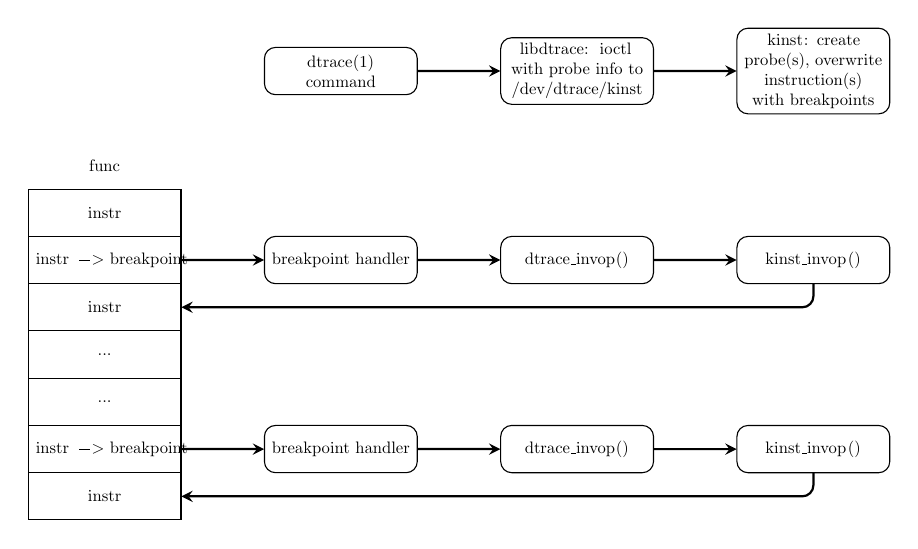
\begin{tikzpicture}[scale=0.6, every node/.style={transform shape}, node distance=1cm]
	\node (header) [header] {\lstinline{func}};
	\node (stack1) [box, below of=header] {\lstinline{instr}};
	\node (stack2) [box, below of=stack1] {\lstinline{instr -> breakpoint}};
	\node (stack3) [box, below of=stack2] {\lstinline{instr}};
	\node (stack4) [box, below of=stack3] {\lstinline{...}};
	\node (stack5) [box, below of=stack4] {\lstinline{...}};
	\node (stack6) [box, below of=stack5] {\lstinline{instr -> breakpoint}};
	\node (stack7) [box, below of=stack6] {\lstinline{instr}};

	\node (dtrace) [func, right of=header, xshift=4cm, yshift=2cm]
		{\lstinline{dtrace(1)} command};
	\node (libdtrace) [func, right of=dtrace, xshift=4cm]
		{libdtrace: \lstinline{ioctl} with probe info to
		\lstinline{/dev/dtrace/kinst}};
	\node (kinst) [func, right of=libdtrace, xshift=4cm]
		{\lstinline{kinst}: create probe(s), overwrite
		instruction(s) with breakpoints};

	\node (trap1) [func, right of=stack2, xshift=4cm] {breakpoint handler};
	\node (dinvop1) [func, right of=trap1, xshift=4cm]
		{\lstinline{dtrace_invop()}};
	\node (kinvop1) [func, right of=dinvop1, xshift=4cm]
		{\lstinline{kinst_invop()}};

	\node (trap2) [func, right of=stack6, xshift=4cm] {breakpoint handler};
	\node (dinvop2) [func, right of=trap2, xshift=4cm]
		{\lstinline{dtrace_invop()}};
	\node (kinvop2) [func, right of=dinvop2, xshift=4cm]
		{\lstinline{kinst_invop()}};

	\draw [arrow] (dtrace) -- (libdtrace);
	\draw [arrow] (libdtrace) -- (kinst);

	\draw [arrow] (stack2) -- (trap1);
	\draw [arrow] (trap1) -- (dinvop1);
	\draw [arrow] (dinvop1) -- (kinvop1);
	\draw [arrow] (kinvop1) |- (stack3);

	\draw [arrow] (stack6) -- (trap2);
	\draw [arrow] (trap2) -- (dinvop2);
	\draw [arrow] (dinvop2) -- (kinvop2);
	\draw [arrow] (kinvop2) |- (stack7);
\end{tikzpicture}
\end{center}

\end{frame}

%\begin{frame}
%\frametitle{Τραμπολίνο}

%\begin{center}
%\begin{tikzpicture}[scale=0.8, every node/.style={transform shape}, node distance=1cm]
	%\node (chunkhdr) [header] {\lstinline{trampchunk}};
	%\node (tramp) [box, below of=chunkhdr] {\lstinline{tramp}};
	%\node (dots) [box, below of=tramp] {...};
	%\node (lasttramp) [box, below of=dots] {\lstinline{tramp}};
	%\node (trampinstr) [box, right of=tramp, xshift=4cm] {\lstinline{instruction}};
	%\node (trampbpt) [box, below of=trampinstr] {\lstinline{breakpoint/jmp}};

	%\node (chunkhdr1) [header, below of=lasttramp] {\lstinline{trampchunk}};
	%\node (dots1) [box, below of=chunkhdr1] {...};

	%\draw [latex-latex] ([xshift=-0.2cm] tramp.west) -- node [auto,swap]
		%{\lstinline{PAGE_SIZE}} ([xshift=-0.2cm] lasttramp.west);
	%\draw [chain] (tramp) -- (trampinstr);
	%\draw [latex-latex] ([xshift=0.2cm] trampinstr.east) -- node
		%[auto,swap,xshift=3.8cm] {\lstinline{KINST_TRAMP_SIZE}}
		%([xshift=0.2cm] trampbpt.east);
%\end{tikzpicture}
%\end{center}

%\end{frame}

%\begin{frame}
%\frametitle{Emulation}

%\begin{itemize}
	%\item Υλοποίηση εντολών assembly στο λογισμικό λόγω αδυναμίας
		%παρακολούθησής τους εντός τραμπολίνου
	%\item Κυρίως στις αρχιτεκτονικές ARM64 και RISC-V
%\end{itemize}

%\end{frame}

\begin{frame}[fragile]
\frametitle{Παρακολούθηση inline συναρτήσεων}

\begin{center}
\begin{tabular}{ll}

Inline function & Non-inline function \\

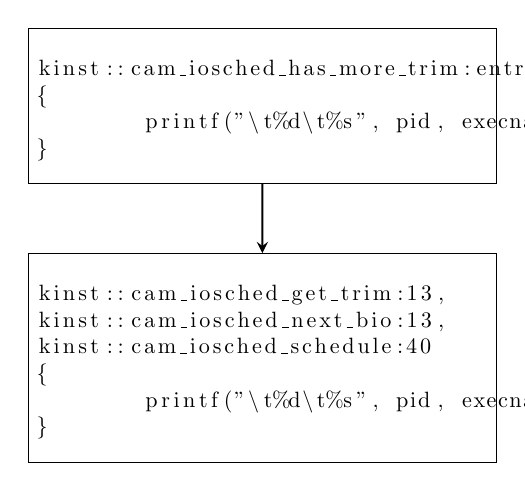
\begin{tikzpicture}[scale=0.8, every node/.style={transform shape}, node distance=1cm]
	\node (initial) [box, text width=7.2cm] {
		\begin{lstlisting}
kinst::cam_iosched_has_more_trim:entry
{
	printf("\t%d\t%s", pid, execname);
}\end{lstlisting}
	};
	\node (outkinst) [box, text width=7.2cm, below of=initial, yshift=-3cm] {
		\begin{lstlisting}
kinst::cam_iosched_get_trim:13,
kinst::cam_iosched_next_bio:13,
kinst::cam_iosched_schedule:40
{
	printf("\t%d\t%s", pid, execname);
}\end{lstlisting}
	};

	\draw [arrow] (initial) -- (outkinst);
\end{tikzpicture} &

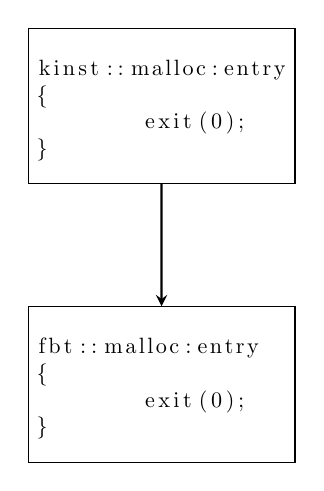
\begin{tikzpicture}[scale=0.8, every node/.style={transform shape}, node distance=1cm]
	\node (initial) [box, text width=4cm] {
		\begin{lstlisting}
kinst::malloc:entry
{
	exit(0);
}\end{lstlisting}
	};
	\node (outkinst) [box, text width=4cm, below of=initial, yshift=-3.42cm] {
		\begin{lstlisting}
fbt::malloc:entry
{
	exit(0);
}\end{lstlisting}
	};

	\draw [arrow] (initial) -- (outkinst);
\end{tikzpicture} \\

\end{tabular}
\end{center}

\end{frame}

\begin{frame}
\frametitle{Πειράματα}

\begin{itemize}
	\item Παρακολούθηση όλων των εντολών μίας συνάρτησης
	\item Παρακολούθηση όλων των εντολών μίας συνάρτησης και εκτύπωση της
		στοίβας κλήσεων
	\item Παρακολούθηση μεμονωμένης εντολής συνάρτησης και εκτύπωση
		καταχωρητή επεξεργαστή
	\item Παρακολούθηση αρχής inline συνάρτησης
	\item Παρακολούθηση τέλους inline συνάρτησης
\end{itemize}

\end{frame}

\begin{frame}

Ευχαριστώ πολύ.

\end{frame}

\end{document}
